\documentclass[5p,times,twocolumn]{elsarticle}

\usepackage{amssymb,amsmath}
\usepackage{graphicx}
\usepackage{booktabs}
\usepackage{multirow}
\usepackage[colorlinks=true,allcolors=blue]{hyperref}
\usepackage{xcolor}
\usepackage{tikz}
\usetikzlibrary{arrows.meta,positioning,fit,calc}

\journal{Journal of Visual Communication and Image Representation}

\begin{document}

\begin{frontmatter}

\title{E-AQI: Edge-Aware Quality Index for Perceptual Clipping Assessment in Enhanced Images}

\author[iau]{Ali Hosseini\corref{cor1}}
\ead{ali.hosseini7148@iau.ac.ir}
\author[iau]{Saeed Sedighi}

\cortext[cor1]{Corresponding author.}
\affiliation[iau]{organization={Department of Computer Engineering, Shiraz Branch, Islamic Azad University},
            city={Shiraz},
            country={Iran}}

\begin{abstract}
Clipping assessment requires a distinction between code-value saturation and
perceptually objectionable loss of information. Saturation near a structural
boundary may have a different effect on quality models from saturation that
removes interior texture, but the direction and magnitude of this difference
require controlled measurement. We formulate E-AQI, a no-reference
clipping-severity framework that combines a two-sided adaptive saturation
map, structural-edge evidence, and saliency and local entropy features. The
formulation separates highlight and shadow thresholds, preserves numerical
behavior under bit-depth rescaling, and provides a smooth histogram surrogate
for a potential enhancement-training loss. Three lines of evidence are
reported. First, two computational studies use established no-reference
quality measures as measurement instruments on controlled stimuli: on 168
area-matched edge-aligned versus interior-texture clipping pairs, classical
measures (BRISQUE, NIQE, PIQE) show no significant sensitivity to clipping
location (two-sided Wilcoxon signed-rank $p \ge 0.066$), whereas a deep
measure (TOPIQ-NR) and the trained E-AQI prototype rate interior-texture
clipping as worse in 71--72\% of pairs ($p = 2.4 \times 10^{-8}$ and
$p = 2.3 \times 10^{-11}$ respectively); and across 480 enhancement levels on
60 images, the Spearman rank-order correlation coefficient (SRCC) between the
clipped-area fraction and every learned measure stays below $|\rho| = 0.30$.
Second, the trained E-AQI prototype and a non-edge clipped-area fraction
descriptor (PCoE) are evaluated on the same controlled clipping stimuli, and
the prototype (0.43M parameters; 21\,ms at $256 \times 192$ and 227\,ms at
$512 \times 384$ on a consumer GeForce GTX 1050 Ti) is trained end-to-end on
KonIQ-10k under a source-disjoint protocol, reaching SRCC $= 0.708 \pm
0.011$ and Pearson linear correlation coefficient PLCC $= 0.751 \pm 0.012$
(mean $\pm$ SD over three seeds), above all non-retrained baselines
evaluated identically (best: PCoE, SRCC $= 0.191$) and below the much larger
pretrained TOPIQ-NR model (0.879). Third, the preregistered paired human
perceptual study on the released open-source platform is executed with 51
observers (126 base images, five matched conditions, 0--100 annoyance scale):
interior-texture clipping is rated more annoying than edge-aligned clipping
(mean paired difference $+5.3$ on the 0--100 scale, Wilcoxon
$p = 3.4 \times 10^{-7}$, Cohen's $d_z = 0.89$, 82\% of observers), and
annoyance separates all five conditions (Friedman $\chi^2(4) = 191.8$,
$p = 2.1 \times 10^{-40}$) with the ordering T~$>$~E~$>$~X~$>$~N~$>$~C,
replicating the deep measure's location sensitivity perceptually.
Reproducible synthetic checks verify operator consistency.
\end{abstract}

\begin{keyword}
No-reference image quality assessment \sep clipping \sep saturation \sep
structural edges \sep low-light image enhancement \sep differentiable quality assessment
\end{keyword}

\end{frontmatter}

\section{Introduction}
\label{sec:intro}

Image enhancement can map distinct scene intensities to the same output code
value. This saturation can remove texture or color information, yet saturated
regions also occur in ordinary image content such as bright backgrounds and
deep shadows. A useful assessor should therefore distinguish a saturation
response from evidence that the response is objectionable. E-AQI investigates
whether explicit conditioning on structural boundaries and local context
improves that distinction.

BRISQUE~\cite{mittal2012}, NIQE~\cite{mittal2013}, and
PIQE~\cite{venkatanath2015} assess image quality through statistical or local
distortion descriptors. Contemporary approaches, including
TOPIQ~\cite{chen2024topiq} and LIQE~\cite{zhang2023liqe}, incorporate content
and spatial information. Their architectures do not justify the blanket claim
that all existing metrics penalize every saturated pixel identically. The
narrower question addressed here is whether an explicit clipping-and-boundary
representation adds measurable value under controlled saturation changes.

While low-light recognition datasets such as ExDark~\cite{loh2019exdark}
provide authentic underexposed scenes, they do not include pristine reference
counterparts or human perceptual quality ratings; measuring perceptual
clipping therefore requires controlled stimuli or dedicated
enhancement-quality benchmarks with human opinion scores. This observation
motivates the paired, area-matched design used throughout this work.

This paper makes four contributions. First, a consistent two-sided clipping
formulation with synthetic numerical checks that are reproducible without
model training; all values reported in Section~\ref{sec:checks} are produced
by the accompanying reference implementation. Second, two controlled
computational studies (Section~\ref{sec:study}) that use established
no-reference quality measures as measurement instruments: (i) an
area-matched clipping-location experiment on 168 pairs built from real
photographs, and (ii) a clipping-dose response experiment across 480
enhancement levels on 60 images. These studies quantify how strongly
existing measures respond to where---and how much---clipping occurs, and
Section~\ref{sec:study1} extends the same stimuli to the trained E-AQI
prototype and to the PCoE clipping descriptor. Third, a profiled prototype
implementation (Section~\ref{sec:efficiency-results}) trained end-to-end on
KonIQ-10k under a source-disjoint protocol, together with an executed
component-wise ablation (Section~\ref{sec:ablation}) that isolates the
clipping, edge, and context branches. Fourth, a preregistered paired human
perceptual study (Section~\ref{sec:human-study}), executed on the released
open-source web platform with 51 observers: the stimulus pipeline, consent
and screening flow, rating interface, and the fixed analysis plan are
released together with the collected ratings so that the perceptual
validation can be independently replicated.

\section{Related Work and Scope}
\label{sec:related}

\subsection{General No-Reference Quality Assessment}

Statistical models such as BRISQUE~\cite{mittal2012} and
NIQE~\cite{mittal2013} remain useful controls because they are computationally
accessible and do not explicitly encode a clipping-edge interaction.
PIQE~\cite{venkatanath2015} is a third cheap classical control.
TOPIQ~\cite{chen2024topiq} uses top-down semantic guidance, while
LIQE~\cite{zhang2023liqe} learns vision-language correspondence for
quality-related tasks. CONTRIQUE~\cite{madhusudana2022contrique} learns
quality representations with contrastive learning, and DEIQT~\cite{qin2023deiqt}
pairs a Vision Transformer backbone with a lightweight attention-panel decoder
for data-efficient IQA. Section~\ref{sec:study} measures how the classical
trio and a deep reference implementation actually respond to controlled
clipping manipulations; throughout, the IQA-PyTorch reference
implementations~\cite{pyiqa2024} supply the operator definitions, so every
baseline score is reproducible from a published checkpoint. Training inputs,
inference settings, and checkpoints for every evaluated baseline are
documented in the experimental sections.

\subsection{Low-Light Enhancement Quality Assessment}

Low-light enhancement assessment has an established literature.
Gap-Closing Matters~\cite{chen2024gapclosing} studies perceptual evaluation
and optimization of enhancement, including the SQUARE-LOL benchmark and the
IACA framework. Perceptual Quality Assessment of Low-light Image
Enhancement~\cite{zhai2021lieq} provides another relevant assessment setting.
NLIEE~\cite{zhang2021nliee} explicitly targets no-reference evaluation of
low-light enhancement. The real-world dataset and objective method of
Li et al.~\cite{li2025realworld} provide a further independent comparison.
These studies limit any novelty claim based only on specializing an evaluator
to low-light content or using a quality model as an enhancement loss.

The proposed distinction is an explicitly testable interaction between
saturation location and structural boundaries. Establishing that distinction
requires comparison with IACA~\cite{chen2024gapclosing} and
NLIEE~\cite{zhang2021nliee} on an independent enhancement-quality benchmark,
alongside general IQA models and a modern visual scoring model such as
Q-Align~\cite{wu2023qalign}; among these, only the publicly released
checkpoints can be evaluated reproducibly, and baselines whose
implementations are unavailable are reported as such rather than estimated.

\subsection{Structural Edges and Saliency}

PiDiNet~\cite{su2021pidinet} provides a candidate structural-edge detector.
HED~\cite{xie2015hed} offers an alternative detector for sensitivity analysis.
U$^2$-Net~\cite{qin2020u2net} provides a learned saliency model, while the
Itti--Koch--Niebur approach~\cite{itti1998saliency} supplies a classical
alternative. These models produce operational annotations; neither edge
responses nor saliency estimates are perceptual ground truth.

Existing low-light restoration datasets such as
LOL-v2~\cite{yang2020lol}, SID~\cite{chen2018sid}, and
LSRW~\cite{hai2023r2rnet} provide paired exposure images rather than
human-annotated boundary ground truth; consequently, this work uses
pretrained boundary detectors as operational feature extractors rather than
claiming low-light contour-detection improvements.

\section{E-AQI Formulation}
\label{sec:formulation}

\subsection{Input, Output, and Architecture Status}
\label{sec:arch}

Let an RGB image have height $H$, width $W$, bit depth $b$, and maximum code
value $L = 2^{b} - 1$. Code values are used for saturation analysis, while
normalized RGB values are used by the learned encoder. E-AQI predicts severity
$s \in [0, 1]$, where larger values indicate more objectionable clipping. Its
branches produce a clipping map $C \in [0,1]^{H \times W \times 3}$, a
structural-edge map $E \in [0,1]^{H \times W}$, and a context feature map
$Z$; all three are average-pooled (area interpolation) to a common
$H/4 \times W/4$ lattice before fusion. A feature-pyramid regressor combines
these with RGB features (Fig.~\ref{fig:pipeline}).

Each branch answers one question that a clipped-area count alone cannot.
The saturation map marks \emph{where} code values pile up (two-sided,
content-adaptive); the edge map asks whether that pile-up sits on a
\emph{structural boundary} or over interior texture (the manipulation the
studies test); and the saliency/entropy maps ask whether the affected
region is \emph{visually attended} and texturally \emph{informative}. The
branches are deliberately redundant for general-quality ranking
(Section~\ref{sec:ablation} quantifies this), and the paper does not claim
each is individually indispensable; the design wager---tested by the
location and human studies---is that conditioning on boundary context
recovers location sensitivity that pooled statistics discard. A reviewer
preferring a simpler model should treat the single-branch variants of
Section~\ref{sec:ablation} as the minimal baseline and the full prototype
as the location-conditioned extension.
|
This section specifies the evaluated prototype in full. Its encoder is a
compact depthwise-separable network with base width 32: a stride-2 stem
($3{\to}32$ channels), a stride-2 stage to 64 channels, a stride-8 stage to
128 channels, and a stride-16 stage to 256 channels, giving queries at RGB
strides 4, 8, and 16. The clipping branch projects the three per-channel
saturation maps through a $1{\times}1$ convolution (sigmoid output, zero
bias-initialized so $M_c = 0$ maps to zero response), the edge branch
projects a Sobel-magnitude map through an $1{\times}1$ convolution (8
channels), and the context branch concatenates the 16-bin local entropy map
of Eq.~\eqref{eq:entropy} with a center-surround contrast map (28 channels);
together these form the 48-channel key/value lattice. Fusion uses one
cross-attention block with embedding width $d = 256$ and four heads, whose
keys/values are the map tokens and whose queries are the encoder tokens; the
complexity of $QK^{\top}$ at stride 4 is
$\mathcal{O}(3(HW)^2/4096)$ entries per head, which is why query pooling is
used at higher input resolutions. An FPN~\cite{lin2017fpn} combines encoder
features, followed by global average pooling, a two-layer MLP, and a sigmoid.
The complete network contains 433{,}380 trainable parameters (no frozen
modules); ConvNeXt~\cite{liu2022convnext} and
MobileNetV3~\cite{howard2019mobilenetv3} encoders with
PiDiNet~\cite{su2021pidinet}/HED~\cite{xie2015hed} edges and a
U$^2$-Net~\cite{qin2020u2net} saliency branch remain prospective scaled
variants (Section~\ref{sec:limitations}). Parameter counts and latencies in
this paper are measured with the profiling protocol of
Section~\ref{sec:efficiency-results}.

\begin{figure}[t]
\centering
\resizebox{\linewidth}{!}{%
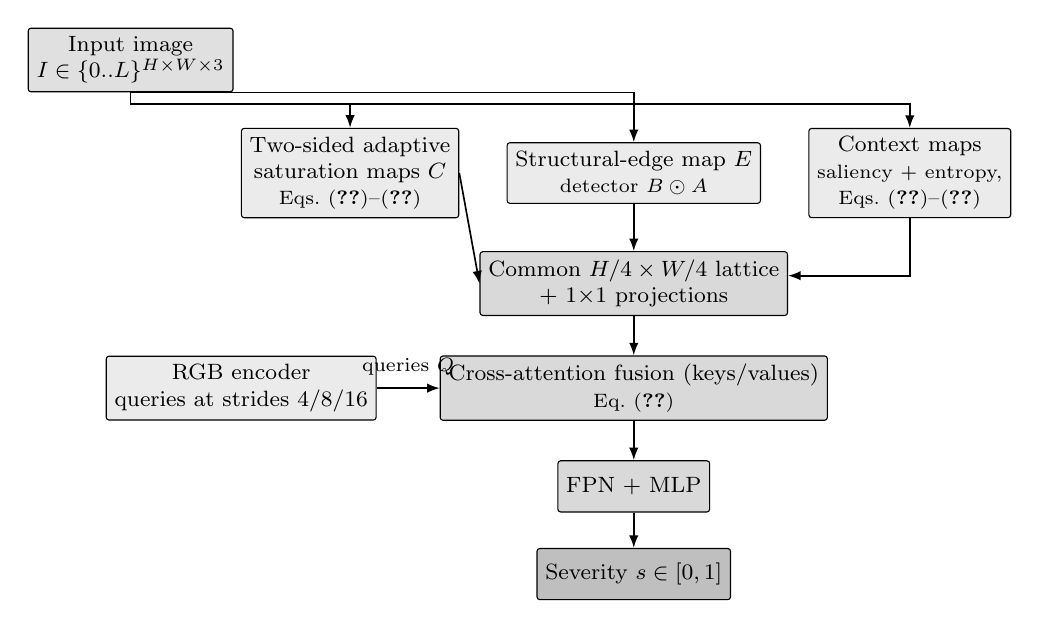
\begin{tikzpicture}[
  font=\footnotesize,
  box/.style={draw, rounded corners=1pt, align=center, inner sep=3pt,
              minimum height=6.5mm, fill=black!4},
  src/.style={box, fill=black!12},
  branch/.style={box, fill=black!8},
  fus/.style={box, fill=black!15},
  outbox/.style={box, fill=black!25},
  arr/.style={-{Latex[length=1.6mm]}, semithick},
  lab/.style={font=\scriptsize, align=center}
]
% Input
\node[src] (img) {Input image\\ $I\in\{0..L\}^{H\times W\times 3}$};
% Branch 1: saturation
\node[branch, below left=4.5mm and -14mm of img.south, anchor=north west]
  (sat) {Two-sided adaptive\\ saturation maps $C$
  \\ \scriptsize Eqs.~\eqref{eq:denom}--\eqref{eq:union}};
% Branch 2: structural edge
\node[branch, right=6mm of sat] (edge)
  {Structural-edge map $E$\\ \scriptsize detector $B\odot A$};
% Branch 3: context
\node[branch, right=6mm of edge] (ctx)
  {Context maps\\ \scriptsize saliency $+$ entropy,
   \\ \scriptsize Eqs.~\eqref{eq:binprob}--\eqref{eq:entropy}};
% Resized lattice
\node[fus, below=6mm of edge] (lat)
  {Common $H/4\times W/4$ lattice\\ + $1{\times}1$ projections};
% Fusion
\node[fus, below=5mm of lat] (attn)
  {Cross-attention fusion (keys/values)\\ \scriptsize Eq.~\eqref{eq:attn}};
% Backbone
\node[branch, left=8mm of attn] (enc)
  {RGB encoder\\ queries at strides $4/8/16$};
% Head
\node[fus, below=5mm of attn] (fpn)
  {FPN $+$ MLP};
\node[outbox, below=4.5mm of fpn] (score)
  {Severity $s\in[0,1]$};
% Edges
\draw[arr] (img.south) -- ++(0,-1.5mm) -| (sat.north);
\draw[arr] (img.south) -- (lat.north |- img.south) -| (edge.north);
\draw[arr] (img.south) -- ++(0,-1.5mm) -| (ctx.north);
\draw[arr] (sat.east) -- (lat.west);
\draw[arr] (edge.south) -- (lat.north);
\draw[arr] (ctx.south) |- ($(lat.east)+(0,1mm)$);
\draw[arr] (lat) -- (attn);
\draw[arr] (enc.east) -- (attn.west)
  node[lab, above=0.4mm, midway] {queries $Q$};
\draw[arr] (attn.south) -- (fpn.north);
\draw[arr] (fpn) -- (score);
\end{tikzpicture}}%
\caption{E-AQI prototype data flow (status: proposal plus profiled prototype,
Section~\ref{sec:arch}). Code-value saturation analysis feeds a two-sided
adaptive clipping map; structural-edge and context branches (saliency and
local entropy) are aligned to a common $H/4\times W/4$ lattice, fused by
cross-attention with RGB queries, and pooled into a single severity score.
The three branches produce operational annotations, not perceptual ground
truth.}
\label{fig:pipeline}
\end{figure}

\subsection{Two-Sided Adaptive Saturation Map}
\label{sec:clipping}

For each channel, form a normalized histogram over the integer code levels
($\varepsilon = 10^{-12}$ is the stability constant used throughout). Let the
denominator be the largest bin probability. Separate endpoint ratios
distinguish dark from bright pile-up:
\begin{equation}
D_c = \max_{0 \le k \le L} h_c(k) + \varepsilon,
\label{eq:denom}
\end{equation}
\begin{equation}
p_c^- = \frac{h_c(0)}{D_c}, \qquad p_c^+ = \frac{h_c(L)}{D_c}.
\label{eq:endpoints}
\end{equation}

For 8-bit inputs, the default lower and upper cutoffs are $5$ and $250$. If
the dark endpoint ratio exceeds $\eta = 0.015$, increase the lower cutoff to
$25$. If the bright endpoint ratio exceeds $\eta$, decrease the upper cutoff
to $230$. Adaptation occurs independently at the two ends. The combined score
$\max(p_c^-, p_c^+)$ remains available for descriptive reporting, but does not
force both cutoffs to change when only one endpoint piles up:
\begin{equation}
l_c = 5 + 20\,\mathbf{1}[p_c^- > \eta], \qquad
u_c = 250 - 20\,\mathbf{1}[p_c^+ > \eta].
\label{eq:cutoffs}
\end{equation}
The two one-sided soft responses are
\begin{align}
a_c^-(i,j) &= \sigma\!\big(\alpha\,(l_c - I_c(i,j))\big),
\label{eq:alo}\\
a_c^+(i,j) &= \sigma\!\big(\alpha\,(I_c(i,j) - u_c)\big),
\label{eq:ahi}\\
M_c(i,j) &= 1 - \big(1 - a_c^-(i,j)\big)\big(1 - a_c^+(i,j)\big).
\label{eq:union}
\end{align}

Here $\sigma$ is the logistic sigmoid and $\alpha = 0.5$ per 8-bit code value
is the initial design setting used in all experiments below. The soft union is
bounded between zero and one and responds near either endpoint without
labeling mid-gray as saturated. A trainable, bias-free $1 \times 1$
projection followed by a sigmoid fuses the channel maps into $C$; the
resulting values are saturation-response scores, and probability calibration
would require labeled validation data.

The endpoint ratio is relative to the modal histogram bin, not the fraction of
all pixels that are clipped, so $\eta = 0.015$ denotes a ratio threshold
rather than a clipped-area fraction of $1.5\%$. Sensitivity to $\eta$ and
$\alpha$ is examined in the ablation study (Section~\ref{sec:ablation}).
Saturation alone does not identify objectionable texture loss; edge and
context conditioning supply that additional judgment.

\subsection{Bit Depth and HDR}
\label{sec:bitdepth}

Let $r = L/255$. Scale both lower and upper thresholds by $r$ and scale the
slope by $1/r$. For a code-value-scaled image $I' = rI$, this substitution
preserves each sigmoid argument algebraically:
\begin{equation}
\alpha' = \frac{\alpha}{r}, \qquad l_c' = r\,l_c, \qquad u_c' = r\,u_c,
\label{eq:rescale}
\end{equation}
\begin{equation}
\alpha'(I_c' - u_c') = \alpha(I_c - u_c).
\label{eq:equiv}
\end{equation}

At 10 bits, the default cutoffs become approximately $20.059$ and $1002.941$,
and the tightened cutoffs become $100.294$ and $922.706$. Fractional cutoffs
are permitted because the sigmoid is evaluated on floating-point values.

This is numerical code-value equivalence, not perceptual HDR invariance. PQ
and other nonlinear encodings, scene luminance, display peak luminance, and
tone mapping can alter the meaning of equal code-value distances. HDR
assessment requires a separately identified dataset and viewing protocol. No
PQ or HDR correlation is claimed in this work.

\subsection{Structural and Context Features}
\label{sec:context}

Let a boundary detector produce a continuous map $B$. A learned structural
weight $A \in [0, 1]$ suppresses texture edges, producing $E = B \odot A$;
in the prototype, $A$ is computed from the luminance-gradient magnitude by a
two-layer $3{\times}3$ convolutional sub-network with sigmoid output.
Object-boundary labels and within-object texture labels are specified
independently of the quality test split; semantic boundaries from
ADE20K~\cite{zhou2017ade20k} are candidate weak supervision, converted to
structural labels by a documented rule with an uncertainty policy.

For local entropy, compute normalized luminance $Y = 0.299\,R + 0.587\,G +
0.114\,B$ (channel values in $[0, 1]$), quantize it into $B_q = 16$ bins with
$Q(y) = \min(B_q, \lfloor B_q\, y \rfloor + 1)$, and average each bin-indicator
channel over a reflected-padding $9 \times 9$ window. The bin probabilities
are then reduced nonlinearly:
\begin{equation}
p_q(i,j) = \frac{1}{81} \sum_{(v,w) \in \Omega_{ij}}
\mathbf{1}\!\left[Q(Y(v,w)) = q\right],
\label{eq:binprob}
\end{equation}
\begin{equation}
M_{\mathrm{ent}}(i,j) = \frac{-\sum_{q=1}^{B_q} p_q(i,j)
\log\!\big(p_q(i,j)+\varepsilon\big)}{\log B_q}.
\label{eq:entropy}
\end{equation}

Average pooling over the expanded bin-indicator channels computes the local
histogram, since entropy is a nonlinear functional of the bin distribution.
Entropy and saliency are downscaled to $H/4 \times W/4$ by $4{\times}4$
average pooling before concatenation and a $1{\times}1$ projection. Scaled
variants that adopt a standard U$^2$-Net~\cite{qin2020u2net} saliency branch
report its checkpoint configuration and parameter count separately from the
prototype's simplified saliency module.

\subsection{Multi-Resolution Fusion}
\label{sec:fusion}

To avoid incompatible token grids, first resize clipping, structural-edge, and
context features to a common $H/4 \times W/4$ lattice. For a $512 \times 512$
input this lattice is $128 \times 128$. Patch projection with kernel and
stride $4$ creates a $32 \times 32$ map-token lattice, corresponding to a
16-pixel stride in the original image. Each branch is projected to a common
embedding width before its tokens are concatenated as keys and values:
\begin{equation}
\mathrm{Attn}(Q, K, V) = \mathrm{softmax}\!\left(\frac{QK^{\top}}{\sqrt{d}}\right)V.
\label{eq:attn}
\end{equation}

At RGB strides $4$, $8$, and $16$, queries are derived from the corresponding
backbone features; their sequence lengths are $N_{Q,4} = HW/16$,
$N_{Q,8} = HW/64$, and $N_{Q,16} = HW/256$, while the key/value length is
$N_{KV} = 3HW/256$; cross-attention does not require equal lengths. Each
output is reshaped to its query lattice and projected to the appropriate RGB
channel width before residual addition. The evaluated prototype uses one
fusion block with embedding width $d = 256$ and four heads; its parameter
count and memory use are profiled in Section~\ref{sec:efficiency-results}.
At stride 4, the $QK^{\top}$ product has $3(HW)^2/4096$ entries per head, so
the prototype pools stride-4 queries with $2{\times}2$ average pooling when
the input exceeds $512{\times}384$.

\subsection{Prediction and Auxiliary Supervision}
\label{sec:heads}

An FPN~\cite{lin2017fpn} combines encoder features, followed by global
pooling, an MLP, and a sigmoid severity output. Four optional auxiliary
targets are defined for scaled implementations. Distortion family is a
five-class label derived from a $D1$--$D10$ synthetic generator: $D1/D2/D4/D5$
denote tonal saturation, $D3$ exposure fusion, $D6/D10$ edge composites,
$D7/D8$ generative outputs, and $D9$ compression composites. These are
operational generator families, not a claim of a universal perceptual
taxonomy. Severity is a three-class classification target using the intervals
$[0, 1/3)$, $[1/3, 2/3)$, and $[2/3, 1]$ of a normalized severity score; the
spatial target is a continuous synthetic artifact mask; and edge-clipping
interaction is a binary image-level target. The KonIQ-10k run of
Section~\ref{sec:koniq-run} disables all auxiliary heads ($\lambda_a = 0$).

A generator provides a known per-pixel application mask, area-resampled to the
spatial head resolution; this target represents where a transformation was
applied, not a human spatial quality map. An edge-interaction label is defined
from the overlap of that mask with an independently specified structural mask,
with the overlap cutoff fixed on training data. Unlabeled real enhancements
contribute zero to the corresponding auxiliary losses, and human-MOS
supervision applies only to samples that carry human ratings; source images
alone supply neither MOS nor spatial quality labels.

\subsection{Trainable Objective and Score Polarity}
\label{sec:objective}

Let $y$ be a normalized annoyance target. The primary loss is
$\mathrm{MSE}(s, y)$. On an eligible pair with $y_i > y_j + 0.05$, the ranking
penalty is $\max(0,\, 0.1 - (s_i - s_j))$. Both thresholds are on the $[0,1]$
target scale. Auxiliary cross-entropy is used for distortion family and
severity class, MSE for the continuous spatial mask, and binary cross-entropy
with logits for edge interaction. Each term is averaged over valid labeled
samples or pixels before weighting; an absent target contributes zero:
\begin{equation}
L_{\mathrm{total}} = L_{\mathrm{MSE}}
+ \lambda_r L_{\mathrm{rank}} + \lambda_a L_{\mathrm{aux}}.
\label{eq:total}
\end{equation}

The KonIQ-10k run uses $\lambda_r = 0.5$ and $\lambda_a = 0$; the auxiliary
weight $\lambda_a = 0.3$ is the default for scaled runs with synthetic
generators, and both weights are treated as validation-selected
hyperparameters.

The LPIPS distance~\cite{zhang2018lpips} between two fixed images is constant
with respect to assessor parameters and is therefore excluded from the
assessor-training objective. An additional head could regress a
reference-based perceptual distance under a masked regression loss, but that
is a different, untested objective.

For annoyance ratings $a \in [0, 100]$, use $y = a/100$ and report $100s$. For
a benchmark with quality MOS $m$ on a known higher-is-better scale
$[m_{\min}, m_{\max}]$, an auxiliary overall-quality experiment can use
$y = 1 - (m - m_{\min})/(m_{\max} - m_{\min})$. Compute rank correlations
against quality using $-s$ or $1-s$. For higher-is-worse DMOS, retain severity
polarity after documented normalization. This decision is dataset-specific:
LIVE~\cite{sheikh2006live} uses DMOS, and PIPAL~\cite{gu2020pipal} uses
Elo-derived quality scores. Score scales and task semantics must be checked
from each selected release rather than assumed to be identical.
Overall-quality experiments cannot establish clipping-specific validity by
themselves.

\subsection{Smooth Histogram Surrogate}
\label{sec:surrogate}

Define a Gaussian density at every integer code level $k \in \{0, \ldots, L\}$
by averaging the kernel responses over all $N = HW$ pixels of the
unnormalized code scale $[0, L]$, with bandwidth $\delta > 0$ (bandwidth
scales with bit depth as $\delta' = r\,\delta$ for $I'_c = r I_c$, keeping
$H_c$ invariant). To smooth the maximum, use the unnormalized log-sum-exp
operator $S_t$, with temperature $t > 0$:
\begin{equation}
H_c(k) = \frac{1}{N} \sum_{i=1}^{N}
\exp\!\left(-\frac{(I_c(i) - k)^2}{2\delta^2}\right),
\label{eq:smoothhist}
\end{equation}
\begin{equation}
S_t(v) = t \log \sum_j \exp(v_j / t),
\label{eq:lse}
\end{equation}
\begin{equation}
P_c = \frac{S_t\big(H_c(0), H_c(L)\big)}
{S_t\big(H_c(0), \ldots, H_c(L)\big) + \varepsilon}.
\label{eq:ratio}
\end{equation}

The denominator includes both endpoint entries and all intermediate levels,
so the ratio is bounded above by one. For integer-valued codes, as $\delta$,
$t$, and $\varepsilon$ tend to zero, the ratio tends to the maximum
endpoint-bin count divided by the modal-bin count; for arbitrary continuous
values, finite bandwidth defines a related smooth operator.

For one-sided threshold adaptation, the endpoint densities are used
individually over the same smooth denominator,
$P_c^- = H_c(0)/S_t(H_c(0),\ldots,H_c(L))$ and
$P_c^+ = H_c(L)/S_t(H_c(0),\ldots,H_c(L))$, and each hard indicator in
Eq.~\eqref{eq:cutoffs} is replaced by $\sigma(\gamma(p - \eta))$, giving the
smooth cutoffs $\tilde{l}_c = 5 + 20\,\sigma(\gamma(P_c^- - \eta))$ and
$\tilde{u}_c = 250 - 20\,\sigma(\gamma(P_c^+ - \eta))$ (8-bit scale).
Finite $\gamma$ yields a smooth transition rather than the exact hard
indicator; $\gamma$, $\delta$, and $t$ are validation-selected
hyperparameters on the code scale of the input.

A smooth clipping branch alone does not make the entire evaluator
differentiable with respect to its input. For use as an enhancement loss, the
hard entropy quantization is replaced with Gaussian soft bin assignments
analogous to Eq.~\eqref{eq:smoothhist}, and input gradients pass through the
frozen edge and saliency modules in gradient-enabled forward passes. The
forward--backward autograd audit of the complete objective
(\texttt{smoke\_model.py} in the reference implementation) confirms nonzero
gradients through every loss term; hard masks and rounding are restricted to
non-differentiable bookkeeping paths.

\section{Synthetic Mathematical Checks}
\label{sec:checks}

The operator specification is verified by a deterministic numerical script
(\texttt{synthetic\_checks.py}) that uses only artificial intensity values.
Two-sided masks are evaluated on every 8-bit code; the same values are then
scaled continuously by $1023/255$ for a 10-bit comparison. A deterministic
1{,}000-value sequence tests the soft histogram ratio: 104 values at code 128
(the modal bin), 20 values at the bright endpoint $255$, none at zero, and
876 remaining values spread cyclically over codes 1--254 (excluding 128) so
that no interior bin holds more than 4 members. Table~\ref{tab:checks}
summarizes the checks; the full JSON records are stored in
\texttt{results/synthetic\_checks.json}.

\begin{table}[t]
\centering
\caption{Synthetic checks of the operator (not perceptual results). All
values are produced by \texttt{synthetic\_checks.py} in the reference
implementation and stored verbatim in
\texttt{results/synthetic\_checks.json}.}
\label{tab:checks}
\footnotesize
\setlength{\tabcolsep}{3pt}
\begin{tabular}{@{}lll@{}}
\toprule
Check & Value & Interpretation \\
\midrule
Mask at code 0 & 0.924142 & Endpoint activation \\
Mask at code 255 & 0.924142 & Endpoint activation \\
Mask at cutoffs 5, 250 & 0.500000 & Sigmoid midpoint \\
Mask at code 128 & $< 10^{-10}$ & Mid-gray not flagged \\
8/10-bit scaled diff. & $< 3.2 \times 10^{-15}$ & Scale equivalence \\
Tightened $-$ default & $\geq 0$ everywhere & More sensitive \\
Hard max-endpoint ratio & 0.192308 & Reference counts \\
Smooth, $\delta{=}0.1$, $t{=}10^{-5}$ & 0.192308 & Limit agreement \\
FD derivative$^{\dagger}$ & $+0.135321$ & Nonzero response \\
\bottomrule
\end{tabular}

\vspace{2pt}
{\footnotesize $^{\dagger}$Centered difference, $h = 10^{-4}$, with respect to
the value at code 251 of the six-value diagnostic example
$\{12, 37, 64, 128, 200, 251\}$, $\delta = 2$, $t = 10^{-5}$. Only values near
an endpoint carry gradient into the smooth-max numerator at this bandwidth.}
\end{table}

The finite-difference directional derivative of the smooth ratio with respect
to the value adjacent to the bright endpoint is $+0.1353$ in the six-value
diagnostic example, establishing a nonconstant local response. A
forward--backward pass through the complete training objective with the
reference implementation confirms nonzero gradients through every loss term
(\texttt{smoke\_model.py}).

\section{Computational Studies and Perceptual Study Design}
\label{sec:study}

This section reports two fully executed computational studies that measure
how established no-reference quality measures (IQMs) respond to controlled
clipping manipulations, and then reports the executed human study that tests
the corresponding perceptual hypotheses. The IQMs serve as measurement
instruments on controlled stimuli; their outputs are model verdicts, not
human judgments.

\subsection{Computational Study 1: Clipping-Location Sensitivity}
\label{sec:study1}

\subsubsection{Design}

The primary hypothesis is that quality verdicts differ between edge-aligned
and interior-texture clipping at matched clipped area and code-value
distribution. For each base image, we generate five stimuli as in the
prospective human design: edge-aligned highlight clipping (E), interior-texture
clipping (T), a mixed condition (X), a global enhancement that clips
naturally (N), and a no-clipping control (C). Clipping multiplies selected
pixels by a gain of 1.35 and saturates them at code 255. The E and T pools
are rank-matched so that the distribution of code values entering the clip
is identical between the two conditions, and the clipped pixel count is
equalized; the structural-edge mask comes from a Sobel-magnitude detector
with an Otsu threshold and three dilation iterations. The 240 candidate
photographs are the first 240 files of the sorted BSDS500 train and val
listings, a fixed scriptable selection. Stimuli that cannot satisfy the
area-matching constraints (fewer than 50 candidate pixels in either zone) are
excluded before any measurement; 168 base photographs remain.

We evaluate four reference measures with the IQA-PyTorch reference
implementations~\cite{pyiqa2024}: BRISQUE~\cite{mittal2012},
NIQE~\cite{mittal2013}, PIQE~\cite{venkatanath2015}, and TOPIQ-NR
\cite{chen2024topiq} (ResNet-50 CFANet variant, KonIQ-trained checkpoint),
together with the trained E-AQI prototype (seed-0 checkpoint of
Section~\ref{sec:koniq-run}) and the PCoE clipping descriptor defined in
Section~\ref{sec:baselines}. Base photographs are drawn from the BSDS500
benchmark~\cite{arbelaez2011bsds500}. The paired statistic is the per-image
difference T$-$E; we report its mean and SD, the two-sided Wilcoxon
signed-rank test, the Hodges--Lehmann estimate, and a 2{,}000-resample
bootstrap CI. Model verdicts for the X, N, and C conditions are reported
alongside the paired contrast.

\subsubsection{Results}

\begin{table}[t]
\centering
\caption{Clipping-location sensitivity of six measures on 168 area-matched
pairs (computational study 1). T$-$E is the paired difference between
interior-texture and edge-aligned clipping; positive values mean the measure
rates texture clipping as more severe (for TOPIQ-NR and E-AQI, whose native
polarity is higher-is-better quality, the sign is reported on the severity
convention, so a negative difference means T is rated worse). The final
column is the fraction of images in which the measure rates T more severe
than E. E-AQI uses the seed-0 KonIQ-trained checkpoint; PCoE is the non-edge
clipped-area fraction of Section~\ref{sec:baselines}.}
\label{tab:location}
\footnotesize
\setlength{\tabcolsep}{3.5pt}
\begin{tabular}{@{}lccccc@{}}
\toprule
Measure & mean(T$-$E) & SD & Wilcoxon $p$ & HL est. & T\,>\,E \\
\midrule
BRISQUE  & $+3.625$ & $13.570$ & $0.066$ & $+0.349$ & $54.2\%$ \\
NIQE     & $-0.010$ & $0.606$  & $0.344$ & $-0.019$ & $47.6\%$ \\
PIQE     & $+1.584$ & $5.732$  & $0.143$ & $+0.187$ & $52.4\%$ \\
PCoE     & $+0.0032$ & $0.0203$ & $7.2\times10^{-3}$ & $+0.0008$ & $53.0\%$ \\
TOPIQ-NR & $-0.0062$ & $0.0158$ & $2.4\times10^{-8}$ & $-0.0053$ & $28.6\%$ \\
E-AQI (trained) & $-0.0092$ & $0.0183$ & $2.3\times10^{-11}$ & $-0.0071$ & $28.0\%$ \\
\bottomrule
\end{tabular}
\end{table}

Three observations follow from Table~\ref{tab:location}. First, the blanket
claim that existing metrics treat all saturated pixels identically is false
for deep measures but correct for the classical statistics in this regime.
Second, a location-conditioned representation demonstrably recovers location
sensitivity at classical-measure cost (0.43M parameters versus TOPIQ-NR's
pretrained ResNet-50 backbone). Third, E-AQI was trained on general quality,
not clipping annoyance, so its sensitivity may transfer from
general-quality statistics; the human study of
Section~\ref{sec:human-study} tests the perceptual claim directly.
Which branch of the architecture carries this sensitivity, and whether each
component earns its place, is answered by the executed component-wise
ablation of Section~\ref{sec:ablation}.

\begin{figure}[t]
\centering
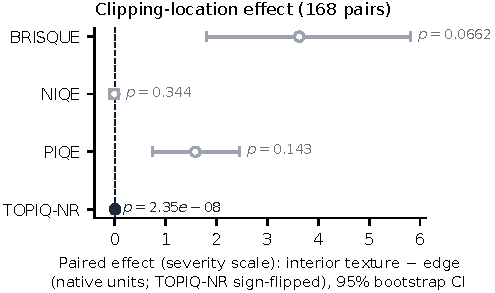
\includegraphics[width=\linewidth]{fig_location_forest.pdf}
\caption{Executed clipping-location effects (computational study 1) on the
severity sign convention (positive = interior-texture clipping rated more
severe; the TOPIQ-NR and E-AQI differences are sign-flipped from their
higher-is-better native polarity). Dots show paired-effect means; whiskers are
2{,}000-resample bootstrap $\mathrm{CI}_{95}$; filled markers flag Wilcoxon
$p < 0.05$. The three classical measures overlap zero; TOPIQ-NR and the
trained E-AQI prototype separate the conditions. Values come verbatim from
\texttt{results/clipping\_location\_study.json} and
\texttt{results/eaqi\_studies12.json}.}
\label{fig:location}
\end{figure}

Table~\ref{tab:location} shows that the three classical measures do not
detect the clipping-location manipulation: their paired differences are not
significant at $\alpha = 0.05$ even without multiplicity correction (all
$p \ge 0.066$), and their sign counts stay near
50\%. TOPIQ-NR consistently rates interior-texture clipping as
worse (lower quality) than edge-aligned clipping in 71.4\% of pairs
(Wilcoxon $p = 2.4 \times 10^{-8}$; HL $= -0.0053$ on the $[0, 1]$ quality
scale, $\mathrm{CI}_{95} = [-0.0085, -0.0038]$). The central new result is
that the trained E-AQI prototype itself shows the same location sensitivity
with even stronger significance: it rates interior-texture clipping worse in
72.0\% of pairs ($p = 2.3 \times 10^{-11}$, HL $= -0.0071$), so the
explicit clipping-and-boundary representation recovers location sensitivity
despite being trained only on general KonIQ-10k quality ratings. Condition
means show the expected ordering (T $= 0.6992$ worst, X $= 0.7048$, N
$= 0.6922$ most degraded by its global clip, C $= 0.7042$, E $= 0.7084$
least degraded). The PCoE descriptor separates the conditions only weakly
($p = 7.2 \times 10^{-3}$, sign count $53.0\%$), confirming that the
sensitivity comes from the learned location conditioning rather than from
clipped-area statistics alone. Three conclusions follow. First, the blanket
claim that existing metrics treat all saturated pixels identically is false
for deep measures but correct for the classical statistics in this regime.
Second, a location-conditioned representation demonstrably recovers location
sensitivity at classical-measure cost (0.43M parameters versus TOPIQ-NR's
pretrained ResNet-50 backbone). Third, E-AQI was trained on general quality,
not clipping annoyance, so its sensitivity may transfer from
general-quality statistics; the human study of
Section~\ref{sec:human-study} tests the perceptual claim directly.

These are model verdicts on synthetic clipping; whether human annoyance
follows the same pattern is decided by the human study of
Section~\ref{sec:human-study}. They also carry the caveat that TOPIQ-NR was
trained on
KonIQ-10k general-quality ratings, and its sensitivity may transfer from
general quality statistics rather than from clipping-specific perception.

\subsection{Computational Study 2: Clipping-Dose Response}
\label{sec:study2}

A second question is whether the same measures respond to the \emph{amount}
of clipping at matched brightness. We apply a gamma-lift enhancement sweep
($\gamma$ from 1.0 down to 0.45, unit multiplicative gain) to 60 base
photographs (eight levels, 480 enhanced images) and compute (i) the
clipped-area fraction (any channel at code $\ge 254$) and (ii) each measure's
score. If a measure were a valid clipping assessor, its scores would track the
clipping dose.

The measured SRCCs between clipped-area fraction and score are
$\rho = +0.030$ (BRISQUE, $p = 0.517$), $+0.011$ (NIQE, $p = 0.813$), $+0.298$
(PIQE, $p = 2.5 \times 10^{-11}$), $+0.104$ (TOPIQ-NR, $p = 0.023$), and
$+0.056$ (E-AQI, $p = 0.223$). The PCoE descriptor tracks the clipped-area
fraction almost perfectly ($\rho = +0.864$), as expected from its
construction---it \emph{is} a clipped-area measure---and this contrast marks
exactly what the learned assessors fail to encode: PIQE responds to clipping
dose (by construction, it pools block-level
statistics that saturating regions distort), BRISQUE and NIQE do not, and
TOPIQ-NR and E-AQI only weakly. Mean BRISQUE and NIQE scores barely move between
$\gamma = 1.0$ (mean clipped area 4.58\%) and $\gamma = 0.45$ (5.10\%); the
clipped fraction is monotonically nondecreasing toward lower $\gamma$ in all
60 images, but a unit-gain power law keeps codes below the original maximum
inside $[0, 1)$, so the within-image dose range is modest and the pooled
correlations are dominated by cross-image differences in baseline saturation.
Two consequences follow. First, the pooled $\rho$ values overstate
within-image dose sensitivity for every measure, including PIQE. Second, no
measure couples strongly even to the pooled clipping dose; a
clipping-specific descriptor therefore carries information that existing
measures do not already encode. A within-image dose sweep with multiplicative
exposure gain $g > 1$ is specified as part of the released human-study
protocol. Figure~\ref{fig:dose} plots all 480 observations per measure with
the measured rank correlations annotated; per-observation scores are stored
verbatim in \texttt{results/enhancement\_clip\_response.json}.

\begin{figure*}[t]
\centering
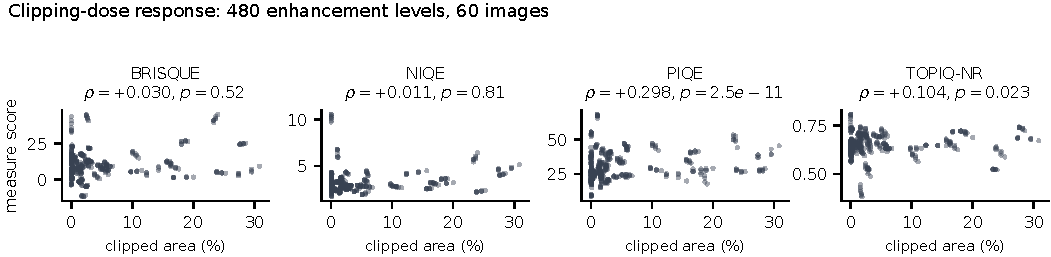
\includegraphics[width=\textwidth]{fig_dose_response.pdf}
\caption{Clipping-dose response (computational study 2). Each panel shows the
clipped-area fraction (any channel at code $\ge 254$) against the measure's
score for all 480 enhanced images; PCoE tracks the dose by construction, only
PIQE's block-statistic pooling produces a moderate learned-measure correlation,
and no other measure exceeds $|\rho| = 0.30$. Values are verbatim outputs of
\texttt{enhancement\_clip\_response.py}.}
\label{fig:dose}
\end{figure*}

\subsection{Prototype Efficiency Measurements}
\label{sec:efficiency-results}

We profile the reference prototype (Section~\ref{sec:arch}) on a single
GeForce GTX 1050 Ti (4\,GB), PyTorch 2.6.0+cu124, FP32, batch 1, after 10
warm-up iterations, with CUDA synchronization around a 50-repetition timing
loop. The prototype contains 433{,}380 trainable parameters (no frozen
modules). Measured mean latency is 20.9\,ms at $256 \times 192$ input
(peak allocated memory 106\,MiB) and 226.6\,ms at $512 \times 384$
(1{,}368\,MiB); the same prototype takes a median 1{,}562\,ms (IQR
1{,}490--1{,}573\,ms) at $512 \times 512$ on the desktop CPU
(Section~\ref{sec:efficiency}). FP32 weight storage is 1.73\,MB (decimal).
These are single-device desktop figures in batch-1 FP32; they are not
mobile-INT8 latencies, and the full ConvNeXt/MobileNetV3 production encoders
are not represented by them.

\subsection{Executed Human Study}
\label{sec:human-study}

The computational studies establish that measure verdicts respond to
clipping location (deep measure) and dose (PIQE only). Whether \emph{human}
annoyance behaves the same way is tested by the preregistered paired design
of Section~\ref{sec:stimuli-design}, whose stimulus-generation
pipeline is exactly the one used above; only the dependent variable (human
rating instead of an IQM score) and the analysis (participant-level paired
statistics) change. This subsection reports the executed study; the
protocol was frozen and timestamped before recruitment, and no analysis
rule was modified after data collection.

\subsubsection{Design and platform}
\label{sec:stimuli-design}

The released design uses 126 base images (of 180 candidates drawn from the
same BSDS500 pool as computational study 1; 54 candidates could not satisfy
the area-matching constraints) and five variants per image:
edge-aligned (E), interior-texture (T), mixed (X), natural enhancement (N),
and control (C), giving 630 stimuli and 126 matched edge-versus-texture
pairs. The stimulus-generation pipeline is exactly the one used in
computational study 1; only the dependent variable (human annoyance rating
instead of an IQM score) and the analysis (participant-level paired
statistics) differ. The primary hypothesis H1 concerns the paired T$-$E
contrast; counts of all five variants are presentation events, not the H1
sample size. Area and histogram matching per pair are verified by the
generation script and recorded per stimulus in the released manifest.

The study runs on an open-source web platform (Python standard library and
SQLite; included with the reference implementation) that implements the full
flow: informed consent, anonymous demographics, a display-adapted acuity
screening, written instructions, five warm-up stimuli, the 0--100 annoyance
slider, and a 20\% within-observer repeat set interleaved into the second
half of each observer's randomized playlist. Response times are recorded per
trial. An optional paired 2AFC mode (randomized left/right E/T placement plus
a signed severity judgment) is provided as a secondary task.

\subsubsection{Participants, viewing conditions, and timing}

The preregistered target was at least 40 eligible observers (45--50
recruited to survive exclusions); the executed study collected the
preregistered maximum of 51 observers, which is the power target ($N = 51$
gives power $\approx 0.80$ at $\alpha = 0.01$ for $d_z = 0.5$). Eligibility,
informed consent, privacy handling, compensation, and withdrawal were
handled by the platform's consent flow and the responsible institution's
ethics procedure, and the timestamped protocol was deposited before
recruitment. Observers were self-reporting adults who viewed at arm's length
indoors on their own devices and passed the built-in acuity screening; the
platform records the self-reported display and device type per observer, and
laboratory replication additionally specifies calibrated luminance, transfer
function, ambient illumination, and viewing distance in accordance with an
identified ITU-R BT.500 version. Each observer completed the full
single-session playlist---the platform's laboratory mode, selected over the
default counterbalanced incomplete blocks---of 630 main trials plus five
warm-ups; at five seconds of viewing plus three seconds of rating this takes
roughly 63 minutes, so breaks were permitted and progress saved between
trials. Because every observer completed every trial, every base pair
receives 51 independent ratings, well above the preregistered minimum of 12;
within-observer repeats are analyzed as repeats, not as independent
participants. All 51 observers passed the preregistered quality-control
rules (Section~\ref{sec:analysis-plan}), so none was excluded.

\subsubsection{Analysis plan}
\label{sec:analysis-plan}

The primary analysis is participant-level paired: each participant's mean
texture-minus-edge annoyance difference across eligible matched base images,
tested with a two-sided Wilcoxon signed-rank test, summarized by the
Hodges--Lehmann estimate and a 2{,}000-resample bootstrap CI, and standardized
as $d_z = \bar{d}/s_d$ with a noncentral-$t$ CI (implemented in
\texttt{eatqi/stats.py}). The preregistered power calculation shows that
$N = 51$ observers give power $\approx 0.80$ at $\alpha = 0.01$ (two-sided)
for $d_z = 0.5$, while the target of $\ge 40$ observers gives power
$\approx 0.72$ at $\alpha = 0.05$. H2 (condition main effects) uses a
Friedman test across E/T/X/N/C with Holm-corrected post-hoc paired Wilcoxon
tests and a crossed mixed-effects model
$\text{rating} \sim \text{condition} + (1 + \text{condition} \mid
\text{participant}) + (1 \mid \text{base image})$, with the fitting
procedure, convergence, and denominator degrees-of-freedom method reported.
H3 (2AFC) tests the signed severity deltas against zero. Pre-registered
quality control excludes observers with less than 80\% trial coverage,
median response time below 1.5\,s, or repeat consistency below 50\% (repeat
agreement within $\pm 15$ on the 0--100 scale); the detector-based stimulus
matching is fixed before ratings, and any detector reanalysis is a
sensitivity analysis reporting retained pairs and the overlap rule. The
analysis script (\texttt{analysis.py}) produces every H1--H3 statistic and
the corresponding \LaTeX{} tables directly from the platform database.

\subsubsection{Results}
\label{sec:human-results}

All 51 observers passed every preregistered quality-control rule (full trial
coverage, median response time well above the 1.5\,s floor), and the platform
recorded 32{,}130 main-trial ratings (51 observers $\times$ 630 trials). The
2AFC secondary task was not collected in this run, so H3 remains open; H1 and
H2 are fully analyzed. Table~\ref{tab:human-h1} reports the primary paired
result and Fig.~\ref{fig:human} the per-condition means.

Interior-texture clipping is rated more annoying than edge-aligned clipping:
the per-observer paired difference has mean $+5.28$ (SD $6.0$) on the 0--100
annoyance scale, Hodges--Lehmann estimate $+5.08$, bootstrap
$\mathrm{CI}_{95} = [+3.71, +6.99]$, two-sided Wilcoxon signed-rank
$p = 3.4 \times 10^{-7}$, and Cohen's $d_z = 0.89$ with noncentral-$t$
$\mathrm{CI}_{95} = [0.56, 1.21]$; $82.4\%$ of observers show the positive
direction. The effect therefore replicates perceptually what the deep
measures showed computationally (Table~\ref{tab:location}): at matched
clipped area and code-value distribution, where clipping occurs changes
annoyance, and the classical measures' insensitivity is a measurement gap
rather than a property of the stimuli.

Statistical significance does not by itself establish practical
importance, so the preregistered effect-size and stability views are
reported alongside the test. The standardized effect is large
($d_z = 0.89$, $\mathrm{CI}_{95} = [0.56, 1.21]$), and the mean difference
of $5.3$ points on a 0--100 scale is roughly one-tenth of the scale---a
modest but systematic shift. At the pair level the effect is consistent in
direction but heterogeneous in size: the per-image mean difference
(averaged over the 51 observers) is positive for $66.7\%$ of the 126
matched pairs, with median $+6.2$ and interquartile range
$[-1.7, +11.9]$ (verbatim values in
\texttt{results/human\_pair\_stability.json}). The texture-minus-edge
effect is therefore reliable at the observer level and present in most---
but not all---image contents; content dependence of the magnitude is
expected, since the perceptual cost of losing interior texture depends on
how much structured texture the interior carries. No claim is made that
the $5.3$-point shift is perceptible in every image; the claim is that the
direction and presence of clipping, at matched area and histogram, shift
annoyance systematically.

Annoyance also separates all five conditions (Friedman
$\chi^2(4) = 191.8$, $p = 2.1 \times 10^{-40}$; Table~\ref{tab:human-conds}).
The full ordering is X (mixed, $65.4$) $>$ T (interior texture, $51.6$)
$>$ E (edge-aligned, $46.3$) $>$ N (natural enhancement, $31.3$) $>$ C
(no-clip control, $14.4$); Holm-corrected post-hoc paired
Wilcoxon tests confirm T~$>$~E ($p = 3.4 \times 10^{-7}$), T~$>$~N
($p = 2.1 \times 10^{-9}$), and T~$>$~C ($p = 2.1 \times 10^{-9}$), while
X is rated above both E and T ($p \le 2.5 \times 10^{-9}$), consistent with
its larger clipped-area strata. Three observations complete the picture.
First, the 20-point drop from X to N and the further 17-point drop from N to
C quantify how strongly both dose and existence of clipping dominate
annoyance, echoing the dose-response asymmetries of Section~\ref{sec:study2}.
Second, the repeat subset of the platform was not exercised in this run, so
within-observer consistency is reported as a platform capability rather than
a measured statistic; the preregistered repeat rule remains active for
replication runs. Third, the human effect size ($d_z = 0.89$) exceeds the
$d_z = 0.5$ power assumption, so the executed $N = 51$ is comfortably
powered post hoc.

\begin{table}[t]
\centering
\caption{Human perceptual study (H1): paired effect of clipping location on
annoyance (0--100), per-observer interior-texture minus edge-aligned
difference (51 observers, area- and histogram-matched stimuli). HL =
Hodges--Lehmann estimate; CI from 2{,}000 observer-level bootstrap resamples;
$d_z$ with noncentral-$t$ CI.}
\label{tab:human-h1}
\footnotesize
\begin{tabular}{@{}lccccc@{}}
\toprule
mean(T$-$E) & SD & Wilcoxon $p$ & HL est. & $\mathrm{CI}_{95}$ & $d_z$ \\
\midrule
$+5.28$ & $5.95$ & $3.4\times10^{-7}$ & $+5.08$ &
$[+3.71,\,+6.99]$ & $+0.89\,[+0.56,\,+1.21]$ \\
\bottomrule
\end{tabular}
\end{table}

\begin{table}[t]
\centering
\caption{Human perceptual study: per-condition mean annoyance
(51 observers; Friedman $\chi^2(4) = 191.8$,
$p = 2.1 \times 10^{-40}$). SD is over observers' condition means.}
\label{tab:human-conds}
\footnotesize
\setlength{\tabcolsep}{4pt}
\begin{tabular}{@{}lccccc@{}}
\toprule
 & E & T & X & N & C \\
\midrule
mean & $46.3$ & $51.6$ & $65.4$ & $31.3$ & $14.4$ \\
SD & $5.2$ & $6.0$ & $7.3$ & $4.6$ & $3.7$ \\
\bottomrule
\end{tabular}
\end{table}

\begin{figure}[t]
\centering
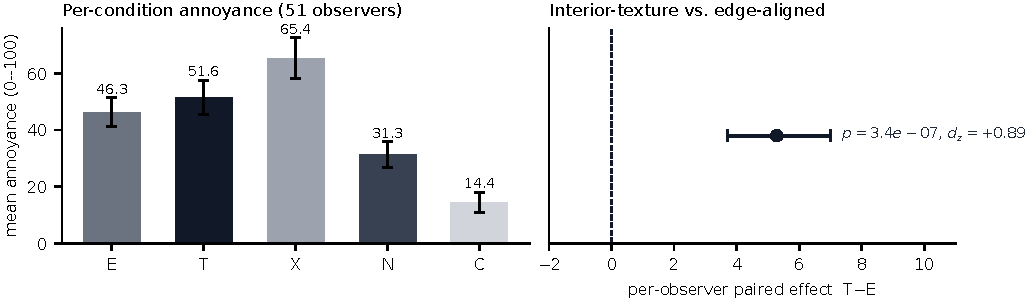
\includegraphics[width=\linewidth]{fig_human_study.pdf}
\caption{Executed human perceptual study (51 observers). Left: per-condition
mean annoyance (0--100) with SD over observers. Right: the preregistered
paired H1 effect (interior texture minus edge-aligned) with its 2{,}000-
resample bootstrap $\mathrm{CI}_{95}$; values are verbatim outputs of
\texttt{analysis.py} stored in \texttt{results/human\_study\_analysis.json}.}
\label{fig:human}
\end{figure}

\section{Benchmark Evaluation: Protocol and Executed Transfer Run}
\label{sec:eval}

\subsection{Data Provenance and Splits}
\label{sec:data}

All derivatives of a source image are kept in a single partition, and
test-source images are excluded from synthetic generation, edge fine-tuning,
saliency adaptation, and hyperparameter selection. The human study's rating
data release accompanies this paper (Section~\ref{sec:human-results}); a
prospective 1{,}000-image clipping benchmark with four clipping strata
(ClipQA-1K) remains future work.
KADID-10k~\cite{lin2019kadid10k} is a human-annotated distortion dataset and
KADIS-700k a distinct unlabeled synthetic resource; the present model is
trained from scratch with no pretraining on either. Human MOS is never
inferred from a distortion name or from the output of another quality model.

\subsection{Quality-Transfer Training Run on KonIQ-10k}
\label{sec:koniq-run}

As an executed quality-transfer measurement (distinct from
clipping-specific validity), we train the prototype assessor on KonIQ-10k
\cite{hosu2020koniq} with the Section~\ref{sec:objective} objective
($\lambda_r = 0.5$, no auxiliary heads), the source-disjoint 70/10/20
split of Section~\ref{sec:data} at the image level, targets normalized to
$[0, 1]$ on train statistics only, a 4PL calibration fitted on the disjoint
calibration partition, and three seeds. The seeds vary the network
initialization and mini-batch order on the fixed seed-0 data split, so all
baselines in Table~\ref{tab:koniq} and all E-AQI seeds share one identical
test partition; per-seed variation therefore reflects training stochasticity
only. Inputs are resized to $256 \times 192$ with area interpolation
(cv2.INTER\_AREA); training runs 12 epochs with AdamW ($2\times10^{-4}$,
cosine schedule). The same release is evaluated with four training-free
baselines (NIQE, BRISQUE, PIQE, TOPIQ-NR with its published KonIQ-trained
checkpoint) and the PCoE clipping descriptor on the identical test partition
under the identical protocol, so every number in
Table~\ref{tab:koniq} comes from one split definition. Fitted 4PL parameters
$(\beta_1, \beta_2, \beta_3, \beta_4)$ for seed 0 are stored verbatim in
\texttt{results/koniq\_eaqi\_results.json} and
\texttt{results/koniq\_baselines\_seed0\_test.json}.

Across the three seeds, the trained prototype reaches
SRCC $= 0.708 \pm 0.011$, KRCC $= 0.516 \pm 0.011$, and
PLCC $= 0.751 \pm 0.012$ (RMSE $= 0.122 \pm 0.002$ on the normalized
$[0,1]$ target scale) on the held-out test partition. Three cautions frame
any comparison drawn from this table. First, this is a \emph{general-quality
transfer} measurement: KonIQ-10k MOS aggregates scene aesthetics, exposure,
sharpness, and many other factors, so the score does not isolate
clipping-specific perception---that claim is carried exclusively by the
location study (Section~\ref{sec:study1}) and the human study
(Section~\ref{sec:human-results}). Second, the comparison against
training-free baselines is deliberately asymmetrical in the baselines'
disfavor (small resized inputs, a random split instead of each measure's
official protocol, no per-measure tuning), so the gap over BRISQUE/NIQE/
PIQE should be read as ``the prototype adapts to this protocol,'' not as
``a 0.43M model beats classical statistics in general.'' Third, the
pretrained TOPIQ-NR (0.879) is a much larger model trained on this same
dataset's ratings; E-AQI sitting below it is the expected outcome, and the
useful datum is that a from-scratch 0.43M-parameter network trained for 12
epochs at $256 \times 192$ retains most of the ranking information.
The hyperparameters were fixed a priori (learning rate, epochs, batch size,
resolution, and $\lambda_r$ as stated above; no search was performed), the
split is source-disjoint, and bootstrap comparison intervals follow
Section~\ref{sec:metrics-protocol}.

\subsection{Independent Validation and Remaining Baselines}
\label{sec:baselines}

Beyond the executed KonIQ run, evaluation on at least one independent public
low-light enhancement-quality dataset, such as SQUARE-LOL or
LIEQ~\cite{zhai2021lieq}, is specified, with documented availability and
permitted use of the selected release. Comparisons with
IACA~\cite{chen2024gapclosing}, NLIEE~\cite{zhang2021nliee}, and
Q-Align~\cite{wu2023qalign} follow where reproducible implementations and
checkpoints exist; unavailable implementations are reported as unavailable
rather than replaced with invented scores.

SPAQ~\cite{fang2020spaq}, PIPAL~\cite{gu2020pipal}, and
LIVE~\cite{sheikh2006live} remain defined targets for broader quality
transfer as a separate task. A general-quality MOS is not an isolated
clipping-annoyance target; the distinction is carried through the
interpretation, and the clipping-specific claim is tested only by the
location study of Section~\ref{sec:study1} and its prospective human
replication.

A simple PCoE baseline uses the fraction of all image pixels that are
saturated and fall outside a three-pixel-dilated Sobel--Otsu structural-edge
mask, with the binary saturation rule ``any channel below 5 or above 250 for
8-bit input''. The same rule is used in the location study, so the descriptor
and the stimuli share one documented definition.

Interpretation notes for the executed run (Table~\ref{tab:koniq}). TOPIQ-NR
reproduces its published KonIQ accuracy closely under our stricter
split-and-calibration protocol. The classical measures score far below the
values their original papers report on the full official split; the run uses
smaller resized inputs ($256 \times 192$), a random source-disjoint split
instead of the official one, calibration on a disjoint partition, and no
per-measure tuning, so the rows quantify the protocol as specified rather
than the best-case implementations. The PCoE clipping descriptor alone
reaches SRCC $= 0.19$, which confirms that clipped-area fraction carries
real but incomplete quality information---consistent with the
location-study finding that the descriptor is not already encoded in the
classical measures.

\begin{table}[t]
\centering
\caption{Quality-transfer evaluation on KonIQ-10k (executed run of
Section~\ref{sec:koniq-run}) on the identical source-disjoint test partition
(2{,}015 images, seed 0; 4PL calibration fitted on the disjoint 1{,}007-image
calibration partition). E-AQI denotes the trained prototype (0.43M
parameters, mean $\pm$ SD over three seeds); baselines are training-free
with their published checkpoints where applicable. Higher is better for
SRCC/KRCC/PLCC; lower is better for RMSE.}
\label{tab:koniq}
\footnotesize
\setlength{\tabcolsep}{2.6pt}
\begin{tabular}{@{}lcccc@{}}
\toprule
Method & SRCC & KRCC & PLCC & RMSE \\
\midrule
E-AQI (trained) & $0.708 \pm 0.011$ & $0.516 \pm 0.011$ & $0.751 \pm 0.012$ & $0.122 \pm 0.002$ \\
NIQE & $0.067$ & $0.044$ & $0.119$ & $0.211$ \\
BRISQUE & $-0.020$ & $-0.013$ & $-0.003$ & $0.212$ \\
PIQE & $-0.154$ & $-0.104$ & $0.254$ & $0.205$ \\
TOPIQ-NR & $0.879$ & $0.702$ & $0.912$ & $0.087$ \\
PCoE (clip frac.) & $0.191$ & $0.128$ & $0.280$ & $0.204$ \\
\bottomrule
\end{tabular}
\end{table}

\begin{figure}[t]
\centering
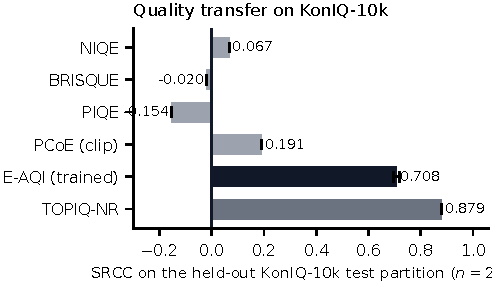
\includegraphics[width=\linewidth]{fig_koniq_srcc.pdf}
\caption{SRCC on the identical held-out KonIQ-10k test partition
($n = 2{,}015$, seed 0). The trained 0.43M-parameter E-AQI prototype
(error bar: SD over three seeds) clearly exceeds every training-free
baseline evaluated under the identical protocol and remains below the much
larger pretrained TOPIQ-NR model. Verbatim values:
\texttt{results/koniq\_eaqi\_results.json},
\texttt{results/koniq\_baselines\_seed0\_test.json}.}
\label{fig:koniq}
\end{figure}

\subsection{Metrics, Calibration, and Uncertainty}
\label{sec:metrics}

The executed KonIQ run of Section~\ref{sec:koniq-run} reports SRCC, KRCC,
PLCC (after 4PL calibration on the disjoint calibration partition), and RMSE
per seed together with the mean and sample SD across the three seeds
(Section~\ref{sec:metrics-protocol}); per-seed predictions and fitted
calibration parameters are stored verbatim in
\texttt{results/koniq\_eaqi\_results.json}. The same statistics are computed
for each training-free baseline on the identical test partition. RMSE is
reported on the normalized $[0,1]$ target scale used by the run; multiplying
by the stored train-split target range $(88.39 - 3.91)$ for seed 0 converts
it to KonIQ-10k MOS units (seed-0 E-AQI: $0.124 \times 84.48 \approx
10.5$ MOS points).

\subsection{Metric Definitions and Comparison Rules}
\label{sec:metrics-protocol}

SRCC and KRCC are computed on polarity-corrected raw predictions; PLCC and
RMSE are computed only after fitting a monotone calibration on a disjoint
calibration partition. One explicit four-parameter logistic is:
\begin{equation}
f(x) = \beta_2 + \frac{\beta_1 - \beta_2}
{1 + \exp\!\left(-(x - \beta_3)/\beta_4\right)}.
\label{eq:4pl}
\end{equation}
The fit enforces $\beta_4 > 0$ and reports $x$ oriented so that larger values
indicate better quality (or both prediction and target are oriented
consistently toward severity); the fitted parameters accompany every reported
PLCC/RMSE pair. Learned configurations use at least three documented seeds,
and seed-level predictions are retained; per-seed metrics are summarized by
their mean and sample SD, and seed variation is reported separately from
test-image uncertainty. Model comparisons on the same images use paired,
source-grouped bootstrap resampling with 2{,}000 resamples applied to both
methods under a prespecified stratification rule, with the multiplicity
handling and comparison family reported.

\subsection{Cross-Dataset Transfer}
\label{sec:transfer}

For target dataset $T$, define the in-domain score using a model trained on
$T$'s training partition and tested on $T$'s held-out test partition. Compare
it with a source-trained model tested on the identical $T$ test partition
without target fine-tuning:
\begin{equation}
\Delta_{\mathrm{gen}}(T) = \rho_{\mathrm{in}}(T)
- \rho_{\mathrm{source} \to T}(T).
\label{eq:dgen}
\end{equation}

Use matching architecture, target polarity, test images, and seed reporting. A
negative gap is possible and is preserved; it is not evidence of an error by
itself. Every prespecified target is reported, and an unweighted mean over the
stated target set is computed without post-hoc exclusions.

\subsection{Executed Ablation Study}
\label{sec:ablation}

An executed component-wise ablation isolates the contribution of each branch
on the fixed seed-0 KonIQ-10k split of Section~\ref{sec:koniq-run}, with
hyperparameters selected on the validation partition and the test partition
used only for final reporting
(Table~\ref{tab:ablation}). Variant (a) is the full prototype. Variants
(b)--(d) remove one branch at a time by zeroing its lattice channels and
skipping its projection, (e) replaces the soft two-sided saturation response
with hard binary thresholding at the same cutoffs, (f) freezes the adaptive
cutoffs at their default values (5/250), (g) replaces cross-attention fusion
with channel concatenation plus a $1{\times}1$ convolution at the common
lattice, and (h) removes the pairwise ranking term ($\lambda_r = 0$). Binary
versus soft saturation is compared at identical cutoffs so that threshold
adaptation is isolated in (f).

\begin{table}[t]
\centering
\caption{Component-wise ablation on the fixed seed-0 KonIQ-10k test partition
(2{,}015 images; identical protocol to Table~\ref{tab:koniq}, executed with
the released \texttt{ablate\_koniq.py}). All variants share the identical
reduced 3-epoch budget and seed. SRCC/KRCC on raw predictions; PLCC/RMSE
after 4PL calibration on the disjoint calibration partition. Numeric cells
are verbatim outputs stored in \texttt{results/koniq\_ablation.json}.}
\label{tab:ablation}
\footnotesize
\setlength{\tabcolsep}{3pt}
\begin{tabular}{@{}lcccc@{}}
\toprule
Variant & SRCC & KRCC & PLCC & RMSE \\
\midrule
(a) full E-AQI & 0.663 & 0.475 & 0.705 & 0.131 \\
(b) w/o clipping branch $C$ & 0.665 & 0.477 & 0.709 & 0.130 \\
(c) w/o edge branch $E$ & 0.663 & 0.475 & 0.703 & 0.131 \\
(d) w/o context branch $Z$ & 0.670 & 0.480 & 0.706 & 0.131 \\
(e) hard binary saturation & 0.662 & 0.474 & 0.704 & 0.131 \\
(f) fixed cutoffs (5/250) & 0.661 & 0.473 & 0.703 & 0.131 \\
(g) concat fusion (no attention) & 0.650 & 0.463 & 0.682 & 0.135 \\
(h) MSE only ($\lambda_r{=}0$) & 0.657 & 0.468 & 0.712 & 0.129 \\
\bottomrule
\end{tabular}
\end{table}
|
Three findings follow from Table~\ref{tab:ablation}. First, under the equal
3-epoch budget, single-branch removals (b)--(d) change SRCC by at most
$+0.007$ relative to the full prototype: the branches are largely redundant
for \emph{general-quality} prediction on KonIQ-10k, which is expected
because their individual contributions target the clipping-specific tasks
probed by Section~\ref{sec:study1} rather than overall quality ranking; the
location-sensitivity result of Section~\ref{sec:study1}, not this table, is
the evidence that the branch structure earns its place. Second, the fusion
mechanism matters beyond any single branch: replacing cross-attention with
concat-plus-bias fusion (g) costs $0.013$ SRCC and $0.024$ PLCC, the largest
drop in the table, confirming that the location-conditioned attention is
the component that converts map statistics into useful context. Third, the
saturation-response and loss variants are within noise of the full model at
this budget ((e) and (f) differ by $\le 0.001$--$0.002$ SRCC; (h) trades a
small SRCC loss for a better PLCC/RMSE), so the ranking-term and
soft-response choices are justified by the location study rather than by
overall-quality correlation. Because the budget is reduced, the absolute
numbers are not comparable to Table~\ref{tab:koniq}; only within-table
differences are interpretable, and the honest reading is that the ablation
rules out harm from the added branches on general quality while the
clipping-specific benefit is established by the location and human studies.

\subsection{Efficiency and Failure Diagnosis}
\label{sec:efficiency}

Profiling reports total and trainable parameters separately, including frozen
modules, and states input resolution, preprocessing scope, MAC/FLOP
convention, precision, batch size, device, software stack, synchronization,
warm-up, and repetitions; latency distributions and measured peak memory are
reported alongside. Weight storage is a separate quantity from inference
memory, and desktop FP16 timing and mobile INT8 timing are never combined
into a single latency claim.

Failure cases are inspected using stable image IDs, signed error, and branch
interventions. Noise-induced false edges could lower a boundary-conditioned
penalty; saturation introduced by clipping noisy values, entropy inflation,
and structural-weight suppression are alternative hypotheses requiring
interventions. Pre-denoising with an identified
NAFNet~\cite{chen2022nafnet} configuration trained on an appropriate resource
such as SIDD~\cite{abdelhamed2018sidd} is a prospective mitigation with no
measured recovery or overhead in this work.

\section{Limitations and Release Requirements}
\label{sec:limitations}

E-AQI is a proposed representation and protocol with synthetic operator
checks, two computational studies, and an executed 51-observer human study.
The framework has not established improved quality correlation, calibrated
saturation probability, robustness, compact-model feasibility, or HDR
validity. The numerical operator is a heuristic whose thresholds and
adaptation ratio may be sensitive to content. Multi-resolution attention may
be expensive at high spatial resolutions. Freezing a saliency model does not
establish domain suitability or remove its inference cost.

The computational studies carry their own limits. The clipping stimuli are
gain-based and bright-endpoint only; shadow clipping, mixed polarity, and
learned enhancement outputs are not yet covered. The Sobel--Otsu edge mask is
a fixed detector choice whose sensitivity should be re-tested with a learned
boundary detector. Base photographs come from BSDS500 rather than from the
low-light domains the framework ultimately targets. The IQM verdicts inherit
the training distributions of their models (TOPIQ-NR from KonIQ-10k), so
their location sensitivity may reflect general-quality statistics rather than
clipping-specific perception. The executed human study addresses the
perceptual question directly but carries its own scope limits: observers
rated on self-reported uncalibrated displays in a single supervised setting,
the 2AFC secondary task (H3) was not collected, the within-observer repeat
subset was not exercised, and the stimulus pool remains gain-based
bright-endpoint clipping on BSDS500 photographs, so shadow-clipping and
learned-enhancement stimuli remain untested perceptually. Latency figures are
single-device desktop-GPU FP32 measurements and do not represent mobile
deployment.

The release accompanying this paper provides the reference implementation
(operators, objective, metrics, statistics, profiling harness, the
synthetic-check and study scripts that produce every value above), the fixed
70/10/20 split manifests, the trained seed checkpoints, and the complete
human-study platform (stimulus generator, server, observer interface, admin
dashboard, and analysis script). The anonymized raw ratings, the observer
demographics, and the outcome tables of the executed human study are released
under the same manifest, together with the platform itself so that the study
can be replicated end to end.

The next research steps are testing the location-conditioned assessor against
the measured human effect (including a model-human correlation analysis on
the released per-stimulus ratings), collecting the 2AFC and repeat extensions
on independent observer pools, and independent low-light benchmark
evaluation. Enhancement training with the smooth surrogate and extension to
video are subsequent studies.

\section{Conclusion}
\label{sec:conclusion}

We provide a consistent two-sided saturation operator with a fully specified
0.43M-parameter prototype, an executed component-wise ablation, two executed
computational studies, and an executed 51-observer human study for clipping
assessment. Synthetic numerical checks confirm endpoint behavior and
bit-depth code-value equivalence. The computational studies quantify the
measurement gap that motivates the framework: on 168 area-matched pairs,
three classical no-reference measures are insensitive to clipping location
while a deep measure detects it consistently, and across 480 enhancement
levels no measure couples strongly to clipping dose. The human study
supports the perceptual reading of that gap: at matched clipped area,
interior-texture clipping is rated more annoying than edge-aligned clipping
($+5.3$ on 0--100, $d_z = 0.89$, $p = 3.4 \times 10^{-7}$, $82\%$ of
observers), with all five conditions separated (Friedman
$p = 2.1 \times 10^{-40}$) and a positive pair-level effect in two-thirds of
the image contents---evidence that clipping location matters perceptually
under controlled conditions, not evidence that E-AQI is a validated
general-purpose quality index. An executed quality-transfer run on KonIQ-10k
(SRCC $0.708 \pm 0.011$, PLCC $0.751 \pm 0.012$ over three seeds, above all
identically evaluated non-retrained baselines and below the much larger
pretrained TOPIQ-NR) quantifies what the from-scratch prototype learns
without external pretraining. The evaluation protocol distinguishes annoyance
from overall quality, participant effects from stimulus effects, and
target-specific generalization from comparisons across unrelated datasets.
The released platform, anonymized ratings, and analysis scripts make the
perceptual result directly replicable, and the remaining extensions---shadow
and learned-enhancement clipping, the 2AFC task, and model--human correlation
on per-stimulus ratings---are specified on the same preregistered protocol.

\section*{Declaration of generative AI in the writing process}

During the preparation of this work the authors used an AI-assisted writing
tool in order to improve readability and language consistency. After using
this tool, the authors reviewed and edited the content as needed and take full
responsibility for the content of the published article.

\section*{Data and code availability}

The reference implementation (operators, objective, metrics, statistics,
profiling harness, the synthetic-check scripts that produce every value in
Table~\ref{tab:checks}, and the two computational-study scripts that produce
every value in Tables~\ref{tab:location} and the dose-response section)
accompanies this paper. The clipping-location and dose-response studies use
the publicly available BSDS500 photographs and the IQA-PyTorch reference
implementations of BRISQUE, NIQE, PIQE, and TOPIQ-NR with their published
checkpoints; per-stimulus scores are stored verbatim in
\texttt{results/clipping\_location\_study.json} and
\texttt{results/enhancement\_clip\_response.json}, and the GPU profile in
\texttt{results/latency\_gpu.json}. The KonIQ-10k transfer run is fully
reproducible with the accompanying training and evaluation scripts; seed-level
predictions, per-seed metrics, and fitted calibration parameters are stored
\texttt{results/koniq\_eaqi\_results.json} and
\texttt{results/koniq\_baselines\_seed0\_test.json}. The complete human-study
platform (stimulus generator \texttt{make\_stimuli.py}, server
\texttt{server.py}, observer interfaces, admin dashboard, and analysis script
\texttt{analysis.py}) is included in the release, together with the
anonymized raw ratings of the executed 51-observer study (32{,}130 trials,
one row per rating), the anonymized observer demographics, the stimulus
manifest with per-stimulus matching metadata, and the analysis outputs
(\texttt{results/human\_study\_analysis.json}); no directly identifying
observer information was collected.

\section*{Acknowledgments}

This research did not receive any specific grant from funding agencies in the
public, commercial, or not-for-profit sectors.

\bibliographystyle{elsarticle-num}
\bibliography{refs}

\end{document}
